\subsection*{Modélisation du jeu}
    % Modélisation du jeu
    \begin{frame}{Modélisation du jeu}
        \begin{block}{Les principaux éléments du jeu sont :}
            \begin{itemize}
                \item \textbf{Player} : représente un joueur
                \item \textbf{Move} : structure les données d'un mouvement
                \item \textbf{Board} : modelise le plateau de jeu
                \item \textbf{State} : représente l'état du jeu
            \end{itemize}
        \end{block}
        \begin{figure}
            \begin{center}
                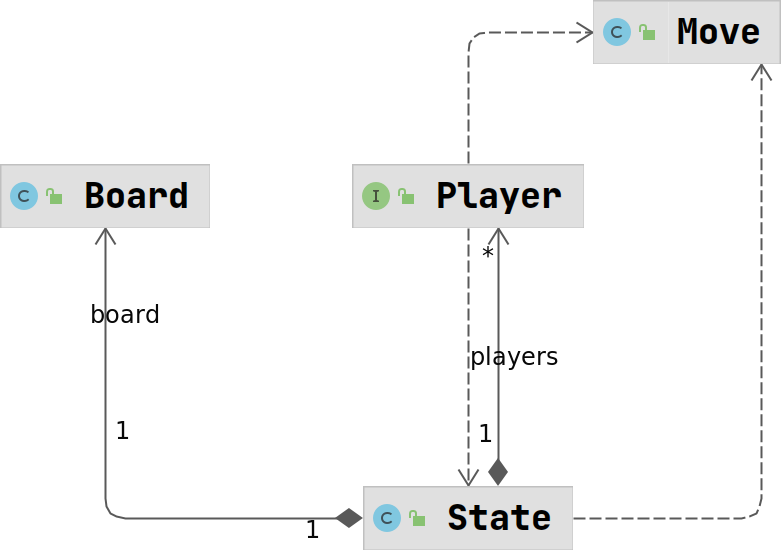
\includegraphics[scale=0.25]{Images/model}
                \caption{Modélisation du jeu}
            \end{center}
        \end{figure}
    \end{frame}

% Interface graphique
\subsection*{Interface graphique}
    % Interface graphique
    \begin{frame}{Mise en place d'une interface graphique}
        \begin{figure}
            \begin{center}
                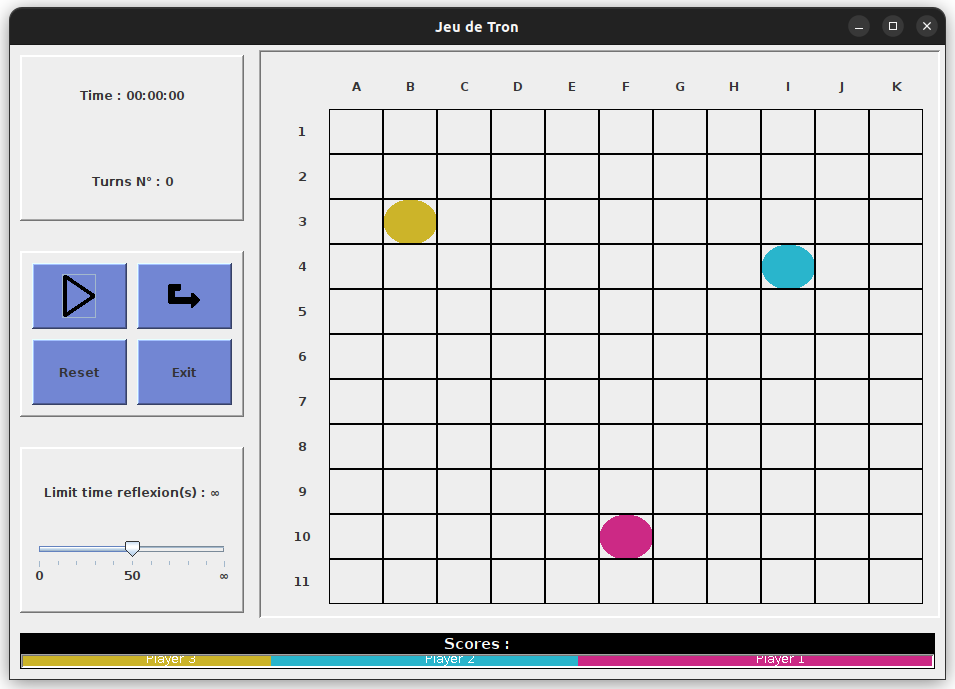
\includegraphics[scale=0.25]{Images/fenetrejeu}
                \caption{Interface graphique}
            \end{center}
        \end{figure}
    \end{frame}

% Fonctionnalités de l'interface graphique
\subsection*{Fonctionnalités}
    % Fonctionnalités de l'interface graphique
    \begin{frame}{Fonctionnalités interface graphique}
        \begin{block}{On peut principalement :}
            \begin{itemize}
                \item \textbf{Lancer une partie} : lancer une partie avec les paramètres choisis
                \item \textbf{Rejouer une partie} : rejouer une partie déjà jouée
                \item \textbf{Changer les paramètres} : changer les paramètres de la partie
            \end{itemize}
        \end{block}
    \end{frame}



